% =====================================================================
\chapter{Técnicas de integração}

A substituição resolve muitas integrais, mas não todas: $\int xe^x\,dx$, $\int\sen^4x\,dx$,
$\int\sqrt{9-x^2}\,dx$ e $\int\frac{dx}{x^2-1}$ pedem outras ferramentas. Este capítulo, adaptado
do capítulo~3 de \emph{Calculus Volume~2}, reúne as quatro técnicas clássicas (integração por
partes, integrais trigonométricas, substituição trigonométrica e frações parciais), os métodos
numéricos para quando nenhuma antiderivada elementar existe e as integrais impróprias, em que
o intervalo ou o integrando são ilimitados.

% ---------------------------------------------------------------------
\section{Integração por partes}\index{integracao por partes@integração por partes}

Integrando a regra do produto $(uv)'=u'v+uv'$, obtemos
\[
\int u\,dv=uv-\int v\,du,\qquad
\int_a^bu\,dv=\Big[uv\Big]_a^b-\int_a^bv\,du .
\]
A ideia é trocar uma integral difícil por outra mais simples. Escolha para $u$ a função que
\emph{simplifica ao derivar} e para $dv$ a que se integra com facilidade. Uma ordem prática
de preferência para $u$ é \textbf{LIATE}\index{liate@LIATE}: \textbf{L}ogaritmos, \textbf{I}nversas trigonométricas,
\textbf{A}lgébricas (polinômios), \textbf{T}rigonométricas, \textbf{E}xponenciais.

\begin{exemplo}{7.1}{Partes}
(a) $\int xe^x\,dx$: $u=x$, $dv=e^xdx$, então $du=dx$, $v=e^x$ e
$\int xe^x\,dx=xe^x-\int e^x\,dx=(x-1)e^x+C$.

(b) $\int\ln x\,dx$: $u=\ln x$, $dv=dx$:
$\ x\ln x-\int x\cdot\frac1x\,dx=x\ln x-x+C$.

(c) $\int x^2\sen x\,dx$ pede partes duas vezes:
$-x^2\cos x+\int2x\cos x\,dx=-x^2\cos x+2x\sen x+2\cos x+C$.

(d) $\int_0^\pi x\sen x\,dx=\big[-x\cos x\big]_0^\pi+\int_0^\pi\cos x\,dx=\pi+0=\pi$.
\end{exemplo}

\textbf{Integrais cíclicas.}\index{integral!ciclica@cíclica} Às vezes a integral original reaparece. Em
$I=\int e^x\sen x\,dx$, partes duas vezes (sempre com $dv=e^xdx$) dá
$I=e^x\sen x-e^x\cos x-I$, e daí $I=\tfrac12e^x(\sen x-\cos x)+C$.

\figtikz{\begin{tikzpicture}
\begin{axis}[painel,width=6.4cm,height=4.6cm,xmin=-0.2,xmax=3.1,ymin=-0.15,ymax=1.3,xtick={1,2.718},xticklabels={$1$,$e$},ytick={1}]
\addplot[fill=azul!25,draw=none,domain=1:2.718,samples=50]{ln(x)} \closedcycle;
\addplot[fill=laranja!30,draw=none,samples=50,domain=0:1] ({exp(x)},{x}) -- (axis cs:0,1) -- (axis cs:0,0) -- cycle;
\addplot[azul,thick,domain=0.4:3,samples=60]{ln(x)};
\draw[dashed] (axis cs:0,1) -- (axis cs:2.718,1) -- (axis cs:2.718,0);
\node[azul,font=\small] at (axis cs:2.25,0.33) {$\int_1^e\!\ln x\,dx$};
\node[laranja!80!black,font=\small] at (axis cs:0.8,0.55) {$\int_0^1\! e^y\,dy$};
\end{axis}\end{tikzpicture}}{Partes, geometricamente: as duas áreas somam o retângulo
$e\times1$, ou seja, $\int_1^e\ln x\,dx=e-\int_0^1e^y\,dy=e-(e-1)=1$.}

% ---------------------------------------------------------------------
\section{Integrais trigonométricas}\index{integrais trigonometricas@integrais trigonométricas}

\textbf{Potências de seno e cosseno}, $\int\sen^mx\cos^nx\,dx$:
\begin{itemize}
\item se uma das potências é \emph{ímpar}, separe um fator dela e converta o resto com
  $\sen^2+\cos^2=1$. Por exemplo, $n$ ímpar: guarde $\cos x\,dx$ e use $u=\sen x$;
\item se ambas são \emph{pares}, reduza o grau com
  $\sen^2x=\frac{1-\cos2x}2$, $\cos^2x=\frac{1+\cos2x}2$, $\sen x\cos x=\frac12\sen2x$.
\end{itemize}

\textbf{Potências de tangente e secante}, $\int\tg^mx\sec^nx\,dx$: se $n$ é par, guarde
$\sec^2x\,dx$ e use $u=\tg x$; se $m$ é ímpar, guarde $\sec x\tg x\,dx$ e use $u=\sec x$
(com $\tg^2=\sec^2-1$). Os demais casos costumam exigir partes, como $\int\sec^3x\,dx$.

\textbf{Produtos com frequências diferentes} usam as fórmulas de produto em soma, por exemplo
$\sen A\cos B=\frac12[\sen(A-B)+\sen(A+B)]$.

\begin{exemplo}{7.2}{Integrais trigonométricas}
(a) $\int\sen^3x\cos^2x\,dx=\int(1-\cos^2x)\cos^2x\sen x\,dx
=-\frac{\cos^3x}3+\frac{\cos^5x}5+C$ \quad ($u=\cos x$).

(b) $\int\cos^2x\,dx=\int\frac{1+\cos2x}2\,dx=\frac x2+\frac{\sen2x}4+C$.

(c) $\int\sen^2x\cos^2x\,dx=\frac14\int\sen^22x\,dx=\frac18\int(1-\cos4x)\,dx
=\frac x8-\frac{\sen4x}{32}+C$.

(d) $\int\sec^3x\,dx$: partes com $u=\sec x$, $dv=\sec^2x\,dx$ dá
$\sec x\tg x-\int\sec x\tg^2x\,dx=\sec x\tg x-\int\sec^3x\,dx+\int\sec x\,dx$, logo
$\int\sec^3x\,dx=\frac12\big(\sec x\tg x+\ln|\sec x+\tg x|\big)+C$.
\end{exemplo}

% ---------------------------------------------------------------------
\section{Substituição trigonométrica}\index{substituicao trigonometrica@substituição trigonométrica}

Raízes de expressões quadráticas desaparecem com a substituição certa, porque
$1-\sen^2=\cos^2$, $1+\tg^2=\sec^2$ e $\sec^2-1=\tg^2$:

\begin{center}\renewcommand{\arraystretch}{1.3}
\begin{tabular}{lll}
\textbf{Expressão} & \textbf{Substituição} & \textbf{Identidade}\\\hline
$\sqrt{a^2-x^2}$ & $x=a\sen\theta$, $-\frac\pi2\le\theta\le\frac\pi2$ & $a^2-a^2\sen^2\theta=a^2\cos^2\theta$\\
$\sqrt{a^2+x^2}$ & $x=a\tg\theta$, $-\frac\pi2<\theta<\frac\pi2$ & $a^2+a^2\tg^2\theta=a^2\sec^2\theta$\\
$\sqrt{x^2-a^2}$ & $x=a\sec\theta$, $0\le\theta<\frac\pi2$ & $a^2\sec^2\theta-a^2=a^2\tg^2\theta$
\end{tabular}\end{center}

Para voltar à variável $x$, desenhe o triângulo retângulo que traduz a substituição.

\figtikz{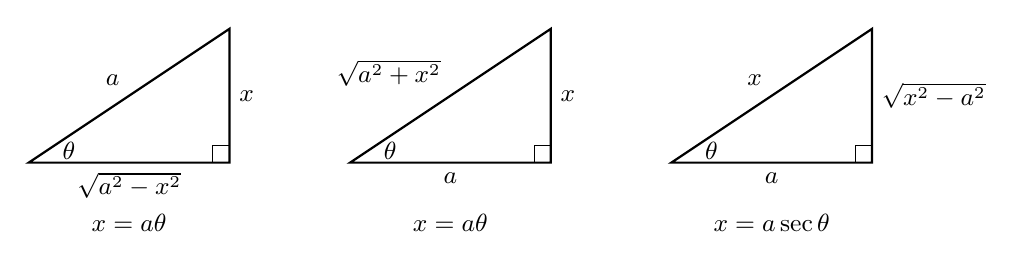
\begin{tikzpicture}[scale=0.85,font=\small]
\draw[thick] (0,0) -- (3,0) -- (3,2) -- cycle; \draw (2.75,0) |- (3,0.25);
\node[below] at (1.5,0) {$\sqrt{a^2-x^2}$}; \node[right] at (3,1) {$x$}; \node[above left] at (1.5,1) {$a$};
\node at (0.6,0.17) {$\theta$}; \node at (1.5,-0.9) {$x=a\sen\theta$};
\begin{scope}[xshift=4.8cm]
\draw[thick] (0,0) -- (3,0) -- (3,2) -- cycle; \draw (2.75,0) |- (3,0.25);
\node[below] at (1.5,0) {$a$}; \node[right] at (3,1) {$x$}; \node[above left] at (1.5,1) {$\sqrt{a^2+x^2}$};
\node at (0.6,0.17) {$\theta$}; \node at (1.5,-0.9) {$x=a\tg\theta$};
\end{scope}
\begin{scope}[xshift=9.6cm]
\draw[thick] (0,0) -- (3,0) -- (3,2) -- cycle; \draw (2.75,0) |- (3,0.25);
\node[below] at (1.5,0) {$a$}; \node[right] at (3,1) {$\sqrt{x^2-a^2}$}; \node[above left] at (1.5,1) {$x$};
\node at (0.6,0.17) {$\theta$}; \node at (1.5,-0.9) {$x=a\sec\theta$};
\end{scope}
\end{tikzpicture}}{Os três triângulos de referência da substituição trigonométrica.}

\begin{exemplo}{7.3}{Substituição trigonométrica}
(a) $\int\sqrt{9-x^2}\,dx$: com $x=3\sen\theta$, $dx=3\cos\theta\,d\theta$ e
$\sqrt{9-x^2}=3\cos\theta$:
\[
\int9\cos^2\theta\,d\theta=\tfrac92(\theta+\sen\theta\cos\theta)+C
=\tfrac92\arcsen\tfrac x3+\tfrac x2\sqrt{9-x^2}+C .
\]
(b) $\int\frac{dx}{x^2\sqrt{x^2+4}}$: com $x=2\tg\theta$, $dx=2\sec^2\theta\,d\theta$, a
integral vira $\frac14\int\frac{\cos\theta}{\sen^2\theta}\,d\theta=-\frac1{4\sen\theta}+C$.
Pelo triângulo, $\sen\theta=\frac x{\sqrt{x^2+4}}$, e o resultado é
$-\frac{\sqrt{x^2+4}}{4x}+C$.
\end{exemplo}

% ---------------------------------------------------------------------
\section{Frações parciais}

Para integrar uma função racional $\frac{P(x)}{Q(x)}$:
\begin{estrategia}{frações parciais}\index{fracoes parciais@frações parciais}
\begin{enumerate}[label=\arabic*.]
\item Se $\operatorname{grau}P\ge\operatorname{grau}Q$, divida primeiro (polinômio + fração
  própria).
\item Fatore $Q$ em fatores lineares $(ax+b)$ e quadráticos irredutíveis $(ax^2+bx+c)$.
\item Escreva uma parcela para cada fator: $\frac A{ax+b}$; para um fator repetido $(ax+b)^k$,
  as parcelas $\frac{A_1}{ax+b}+\dots+\frac{A_k}{(ax+b)^k}$; para um quadrático,
  $\frac{Bx+C}{ax^2+bx+c}$.
\item Encontre as constantes (substituindo raízes ou comparando coeficientes) e integre cada
  parcela: logaritmos, potências e arco-tangentes.
\end{enumerate}
\end{estrategia}

\begin{exemplo}{7.4}{Os três casos}
(a) $\frac{x+5}{x^2+x-2}=\frac A{x-1}+\frac B{x+2}$. Então $x+5=A(x+2)+B(x-1)$; com $x=1$,
$A=2$; com $x=-2$, $B=-1$. Logo
$\int\frac{x+5}{x^2+x-2}\,dx=2\ln|x-1|-\ln|x+2|+C$.

(b) $\frac1{x^2(x+1)}=\frac Ax+\frac B{x^2}+\frac C{x+1}$ dá $B=1$, $C=1$, $A=-1$:
$\int\frac{dx}{x^2(x+1)}=-\ln|x|-\frac1x+\ln|x+1|+C$.

(c) $\frac{2x^2-x+4}{x^3+4x}=\frac Ax+\frac{Bx+C}{x^2+4}$ dá $A=1$, $B=1$, $C=-1$:
\[
\int\frac{2x^2-x+4}{x^3+4x}\,dx=\ln|x|+\tfrac12\ln(x^2+4)-\tfrac12\arctg\tfrac x2+C .
\]
\end{exemplo}

% ---------------------------------------------------------------------
\section{Integração numérica}

Funções como $e^{-x^2}$, $\frac{\sen x}x$ e $\sqrt{1+x^3}$ não têm antiderivada elementar. Com
$\Delta x=\frac{b-a}n$ e $x_i=a+i\Delta x$:
\begin{itemize}
\item \textbf{Regra do trapézio:}\index{regra do trapezio@regra do trapézio}
  $T_n=\frac{\Delta x}2\big[f(x_0)+2f(x_1)+\dots+2f(x_{n-1})+f(x_n)\big]$.
\item \textbf{Regra de Simpson}\index{regra de simpson@regra de Simpson} ($n$ par), que aproxima $f$ por parábolas a cada dois
  subintervalos:
  $S_n=\frac{\Delta x}3\big[f(x_0)+4f(x_1)+2f(x_2)+4f(x_3)+\dots+4f(x_{n-1})+f(x_n)\big]$.
\end{itemize}

\begin{teorema}[Limitantes de erro]{7.1}\index{integracao numerica@integração numérica}
Se $|f''|\le K$ em $[a,b]$, então $|E_T|\le\dfrac{K(b-a)^3}{12n^2}$. Se $|f^{(4)}|\le M$, então
$|E_S|\le\dfrac{M(b-a)^5}{180n^4}$.
\end{teorema}

Dobrar $n$ divide o erro do trapézio por cerca de $4$ e o de Simpson por cerca de $16$.
Simpson é exata para polinômios de grau até $3$.

\figtikz{\begin{tikzpicture}
\begin{axis}[painel,width=7.4cm,height=4.6cm,xmin=0.8,xmax=2.15,ymin=0,ymax=1.15,xtick={1,1.25,1.5,1.75,2},ytick={0.5,1},xticklabel style={font=\tiny}]
\addplot[fill=laranja!25,draw=laranja] coordinates {(1,0) (1,1) (1.25,0.8) (1.5,0.6667) (1.75,0.5714) (2,0.5) (2,0)} -- cycle;
\addplot[azul,thick,domain=0.85:2.1,samples=50]{1/x};
\foreach \a in {1.25,1.5,1.75}{\edef\tmp{\noexpand\draw[laranja] (axis cs:\a,0) -- (axis cs:\a,{1/\a});}\tmp}
\end{axis}\end{tikzpicture}}{Regra do trapézio com $n=4$ para $\int_1^2\frac{dx}x$: os
trapézios ficam acima da curva convexa e superestimam a integral.}

\begin{exemplo}{7.5}{Trapézio $\times$ Simpson}
Para $\int_1^2\frac{dx}x=\ln2\approx0{,}693147$, com $n=4$:
$T_4\approx0{,}697024$ (erro $\approx3{,}9\times10^{-3}$) e $S_4\approx0{,}693254$ (erro
$\approx1{,}1\times10^{-4}$). O teorema garante $|E_T|\le\frac{2\cdot1}{12\cdot16}\approx0{,}0104$
(pois $f''=\frac2{x^3}\le2$), e o erro real é bem menor que essa cota.
\end{exemplo}

% ---------------------------------------------------------------------
\section{Integrais impróprias}\index{integral!impropria@imprópria}

\begin{definicao}
(i) Intervalo infinito: $\displaystyle\int_a^\infty f(x)\,dx=\lim_{t\to\infty}\int_a^tf(x)\,dx$
(analogamente em $-\infty$). Para $\int_{-\infty}^\infty$, divida em um ponto $c$ e exija que
\emph{as duas} partes convirjam.

(ii) Integrando ilimitado: se $f$ é descontínua em $b$,
$\displaystyle\int_a^bf(x)\,dx=\lim_{t\to b^-}\int_a^tf(x)\,dx$ (analogamente em $a$ ou num ponto
interior, dividindo o intervalo).

Se o limite existe e é finito, a integral \textbf{converge}; caso contrário, \textbf{diverge}.
\end{definicao}

\begin{exemplo}{7.6}{Convergência e divergência}
(a) $\int_1^\infty\frac{dx}{x^2}=\lim_{t\to\infty}\big(1-\frac1t\big)=1$, mas
$\int_1^\infty\frac{dx}x=\lim\ln t=\infty$. Em geral, $\int_1^\infty\frac{dx}{x^p}$ converge
(para $\frac1{p-1}$) se, e só se, $p>1$.

(b) $\int_0^1\frac{dx}{\sqrt x}=\lim_{t\to0^+}(2-2\sqrt t)=2$; já $\int_0^1\frac{dx}{x^p}$
converge se, e só se, $p<1$.

(c) $\int_{-\infty}^\infty\frac{dx}{1+x^2}=\frac\pi2+\frac\pi2=\pi$.

(d) \emph{Armadilha:} $\int_{-1}^1\frac{dx}{x^2}$ não vale $\big[-\frac1x\big]_{-1}^1=-2$
(uma integral de função positiva não pode ser negativa!). O integrando explode em $x=0$, e
$\int_0^1\frac{dx}{x^2}$ diverge.
\end{exemplo}

\begin{teorema}[Teste da comparação]{7.2}\index{teste!da comparacao@da comparação}
Se $0\le f(x)\le g(x)$ para $x\ge a$: se $\int_a^\infty g$ converge, então $\int_a^\infty f$
converge; se $\int_a^\infty f$ diverge, então $\int_a^\infty g$ diverge.
\end{teorema}
Por exemplo, $\int_1^\infty e^{-x^2}dx$ converge, pois $e^{-x^2}\le e^{-x}$ para $x\ge1$; e
$\int_1^\infty\frac{1+\sen^2x}{\sqrt x}\,dx$ diverge, pois o integrando é $\ge\frac1{\sqrt x}$.

% ---------------------------------------------------------------------
\section*{Resumo do capítulo}\markright{Resumo do capítulo}
\addcontentsline{toc}{section}{Resumo do capítulo}
\begin{itemize}
\item Partes: $\int u\,dv=uv-\int v\,du$; $u$ pela ordem LIATE; integrais cíclicas voltam a si
  mesmas.
\item Trigonométricas: potência ímpar → guarde um fator; pares → ângulo duplo;
  $\tg^m\sec^n$ → $u=\tg x$ ($n$ par) ou $u=\sec x$ ($m$ ímpar).
\item Substituição trigonométrica: $a\sen\theta$, $a\tg\theta$, $a\sec\theta$ para
  $\sqrt{a^2-x^2}$, $\sqrt{a^2+x^2}$, $\sqrt{x^2-a^2}$; volte pelo triângulo.
\item Frações parciais: divida se for imprópria, fatore, uma parcela por fator (repetidos e
  quadráticos têm forma própria).
\item Trapézio (erro $\sim\frac1{n^2}$) e Simpson (erro $\sim\frac1{n^4}$).
\item Impróprias: limite de integrais próprias; $\int_1^\infty x^{-p}$ converge sse $p>1$;
  $\int_0^1x^{-p}$ converge sse $p<1$; teste da comparação.
\end{itemize}

% Gerado por ferramentas/gerar.py; não edite à mão.
\section*{Exercícios}
\addcontentsline{toc}{section}{Exercícios}
Os pontos antes de cada número indicam a dificuldade: \nivel{1} fácil, \nivel{2} médio, \nivel{3} difícil e \nivel{4} desafio. Os exercícios marcados com \estrela{} têm solução completa, com animação do gráfico, no repositório do livro: \url{https://github.com/AleffAzevedo/calculo-1-pt/blob/main/exercicios/cap7/README.md}. As respostas estão no fim do capítulo.

\begin{itemize}[leftmargin=5.2em,labelsep=0.6em,itemsep=4pt]
\item[\exnum{1}{7.1}] Calcule $\displaystyle\int x\cos x\,dx$ e $\displaystyle\int xe^{-x}\,dx$.
\item[\exnum{1}{7.2}] Calcule $\displaystyle\int x\ln x\,dx$.
\item[\exnum{1}{7.3}] Calcule $\displaystyle\int\tan^{-1}x\,dx$ (use $dv=dx$).
\item[\exnum{1}{7.4}] Calcule $\displaystyle\int_0^{\pi/2}x\sin x\,dx$.
\item[\exnum{1}{7.5}] Calcule $\displaystyle\int\sin^3x\,dx$.
\item[\exnum{1}{7.6}] Calcule $\displaystyle\int\cos^2x\,dx$ e $\displaystyle\int_0^\pi\sin^2x\,dx$.
\item[\exnum{1}{7.7}] Calcule $\displaystyle\int\sin^2x\cos^3x\,dx$.
\item[\exnum{1}{7.8}] Calcule $\displaystyle\int\tan^2x\,dx$ e $\displaystyle\int\sec^4x\,dx$.
\item[\exnum{1}{7.9}] Calcule $\displaystyle\int\sin3x\cos2x\,dx$ usando produto em soma.
\item[\exnum{1}{7.10}] Calcule $\displaystyle\int_0^2\sqrt{4-x^2}\,dx$ com $x=2\sin\theta$ e confira com a área de um quarto de círculo.
\item[\exnum{1}{7.11}] Calcule $\displaystyle\int\frac{dx}{(x^2+9)^{3/2}}$ com $x=3\tan\theta$.
\item[\exnum{1}{7.12}] Calcule $\displaystyle\int\frac{dx}{(x-1)(x+2)}$.
\item[\exnum{1}{7.13}] Calcule $\displaystyle\int\frac{3x+1}{x^2-1}\,dx$.
\item[\exnum{1}{7.14}] Calcule $\displaystyle\int\frac{x^3}{x-1}\,dx$ (divida primeiro).
\item[\exnum{1}{7.15}] Calcule $T_4$ e $S_4$ para $\int_0^2x^3\,dx$ e compare com o valor exato. Por que $S_4$ acerta?
\item[\exnum{1}{7.16}] Decida se convergem e calcule quando for o caso: $\int_1^\infty\frac{dx}{x^3}$ e $\int_1^\infty\frac{dx}{\sqrt x}$.
\item[\exnum{1}{7.17}] Calcule $\int_0^\infty e^{-2x}\,dx$ e $\int_0^1\ln x\,dx$.
\item[\exnum{1}{7.18}] Calcule $\int_0^4\frac{dx}{\sqrt{4-x}}$ e decida se $\int_0^2\frac{dx}{(x-1)^2}$ converge.
\item[\exnum{1}{7.19}] Calcule $\displaystyle\int x^2\sin x\,dx$ e confira derivando a resposta.
\item[\exnum{1}{7.20}] Calcule $\displaystyle\int e^x\cos x\,dx$ (integral cíclica).
\item[\exnum{2}{7.21}] \estrela\ \textbf{Partes com logaritmo (e a figura do retângulo).} Calcule $\int_1^e\ln x\,dx$ e $\int_1^ex\ln x\,dx$ por partes. Interprete o primeiro resultado como
uma diferença de áreas num retângulo.
\item[\exnum{2}{7.22}] \estrela\ \textbf{Uma integral que volta a si mesma.} Calcule $\int e^x\sin x\,dx$ e depois $\int_0^\pi e^x\sin x\,dx$.
\item[\exnum{2}{7.23}] \estrela\ \textbf{A integral da secante ao cubo.} Mostre que $\int\sec^3x\,dx=\frac12\big(\sec x\tan x+\ln|\sec x+\tan x|\big)+C$ e calcule
$\int_0^{\pi/4}\sec^3x\,dx$.
\item[\exnum{2}{7.24}] \estrela\ \textbf{A área da elipse.} Use substituição trigonométrica para mostrar que a elipse $\frac{x^2}{a^2}+\frac{y^2}{b^2}\le1$ tem área $\pi ab$.
\item[\exnum{2}{7.25}] \estrela\ \textbf{Frações parciais com fator repetido.} Calcule $\displaystyle\int\frac{5x^2+3x-2}{x^3+2x^2}\,dx$ e depois a integral de $1$ a $2$.
\item[\exnum{2}{7.26}] \estrela\ \textbf{Trapézio e Simpson para $e^{-x^2}$.} A função $e^{-x^2}$ não tem antiderivada elementar. Calcule $T_4$ e $S_4$ para $\int_0^1e^{-x^2}dx$ e
use os limitantes de erro (com $|f''|\le2$ e $|f^{(4)}|\le12$ em $[0,1]$) para dizer quantas casas são confiáveis.
\item[\exnum{2}{7.27}] Calcule $\displaystyle\int x^2\cos x\,dx$.
\item[\exnum{2}{7.28}] Calcule $\displaystyle\int x^3e^{x^2}\,dx$ (substituição e depois partes).
\item[\exnum{2}{7.29}] Calcule $\displaystyle\int\sin^{-1}x\,dx$ e $\displaystyle\int(\ln x)^2\,dx$.
\item[\exnum{2}{7.30}] Calcule $\displaystyle\int\sin^4x\,dx$.
\item[\exnum{2}{7.31}] Calcule $\displaystyle\int\tan^3x\sec^3x\,dx$.
\item[\exnum{2}{7.32}] Calcule $\displaystyle\int\frac{\sqrt{x^2-9}}{x}\,dx$ ($x>3$).
\item[\exnum{2}{7.33}] Calcule $\displaystyle\int\frac{x^2}{\sqrt{9-x^2}}\,dx$.
\item[\exnum{2}{7.34}] Calcule $\displaystyle\int\frac{x^2+1}{x(x-1)^2}\,dx$.
\item[\exnum{2}{7.35}] Calcule $\displaystyle\int\frac{4}{x^3+4x}\,dx$.
\item[\exnum{2}{7.36}] Calcule $\displaystyle\int\frac{dx}{e^x+1}$ (faça $u=e^x$ e use frações parciais).
\item[\exnum{2}{7.37}] Calcule $S_4$ para $\int_0^\pi\sin x\,dx$. Qual o menor $n$ que garante, pelo teorema, erro de Simpson menor que $10^{-6}$?
\item[\exnum{2}{7.38}] Calcule $\int_0^\infty xe^{-x}\,dx$ e $\int_{-\infty}^\infty\frac{dx}{x^2+4x+5}$.
\item[\exnum{2}{7.39}] Calcule $\int_0^3\frac{dx}{(x-1)^{2/3}}$ (cuidado com $x=1$).
\item[\exnum{2}{7.40}] Use comparação para decidir: $\int_1^\infty\frac{dx}{x^2+\sqrt x}$ e $\int_2^\infty\frac{dx}{\ln x}$.
\item[\exnum{3}{7.41}] \estrela\ \textbf{O comprimento da parábola.} Calcule o comprimento de arco de $y=x^2$ para $0\le x\le1$.
\item[\exnum{3}{7.42}] \estrela\ \textbf{A trombeta de Gabriel.} Gire $y=\frac1x$, $x\ge1$, em torno do eixo $x$. Mostre que o sólido tem volume finito, mas a
superfície tem área infinita.
\item[\exnum{3}{7.43}] \estrela\ \textbf{A função gama.} Seja $\Gamma(x)=\int_0^\infty t^{x-1}e^{-t}\,dt$ para $x>0$. Mostre que $\Gamma(1)=1$, que
$\Gamma(x+1)=x\,\Gamma(x)$ e conclua que $\Gamma(n+1)=n!$.
\item[\exnum{3}{7.44}] \estrela\ \textbf{A substituição universal $t=\tan(x/2)$.} Com $t=\tan\frac x2$, mostre que $\cos x=\frac{1-t^2}{1+t^2}$ e $dx=\frac{2\,dt}{1+t^2}$, e calcule
$\displaystyle\int_0^{\pi/2}\frac{dx}{2+\cos x}$.
\item[\exnum{3}{7.45}] \estrela\ \textbf{Crescimento logístico.} Uma população segue $\dfrac{dP}{dt}=0{,}5\,P\Big(1-\dfrac P{1000}\Big)$, com $P(0)=100$. Separe as variáveis,
use frações parciais e encontre $P(t)$. Quando a população chega a $500$? Quando cresce mais rápido?
\item[\exnum{3}{7.46}] Calcule $\displaystyle\int e^{2x}\sin3x\,dx$.
\item[\exnum{3}{7.47}] Calcule $\displaystyle\int\cos\sqrt x\,dx$.
\item[\exnum{3}{7.48}] Deduza a fórmula de redução $\int\sin^nx\,dx=-\frac1n\sin^{n-1}x\cos x+\frac{n-1}n\int\sin^{n-2}x\,dx$ e calcule $\int_0^{\pi/2}\sin^6x\,dx$.
\item[\exnum{3}{7.49}] Calcule $\displaystyle\int x\tan^{-1}x\,dx$.
\item[\exnum{3}{7.50}] Calcule $\displaystyle\int\frac{dx}{(1+x^2)^2}$ e $\displaystyle\int_0^1\frac{dx}{(1+x^2)^2}$.
\item[\exnum{3}{7.51}] Calcule $\displaystyle\int\frac{e^x}{e^{2x}+3e^x+2}\,dx$.
\item[\exnum{3}{7.52}] Calcule $\displaystyle\int\frac{x^3+x+1}{(x^2+1)^2}\,dx$.
\item[\exnum{3}{7.53}] Calcule $\displaystyle\int\frac{dx}{x^3+1}$.
\item[\exnum{3}{7.54}] Calcule $\displaystyle\int\frac{\sqrt x}{1+x}\,dx$ (racionalize com $u=\sqrt x$).
\item[\exnum{3}{7.55}] Quantos subintervalos garantem, pela regra do trapézio, erro menor que $10^{-4}$ em $\int_1^2\frac{dx}x$?
\item[\exnum{3}{7.56}] Calcule $\int_0^\infty e^{-x}\sin x\,dx$.
\item[\exnum{3}{7.57}] Calcule $\int_1^\infty\frac{\ln x}{x^2}\,dx$.
\item[\exnum{3}{7.58}] Para quais $p$ a integral $\int_0^1\frac{dx}{x^p}$ converge, e para quanto? E $\int_0^\infty\frac{dx}{x^p}$?
\item[\exnum{3}{7.59}] Calcule $\displaystyle\int_0^\infty\frac{dx}{(1+x)\sqrt x}$ (é imprópria nas duas pontas).
\item[\exnum{3}{7.60}] A transformada de Laplace de $f$ é $F(s)=\int_0^\infty e^{-st}f(t)\,dt$. Calcule-a para $f(t)=1$ e $f(t)=t$ ($s>0$).
\item[\exnum{4}{7.61}] Prove que $\displaystyle\int_0^1\frac{x^4(1-x)^4}{1+x^2}\,dx=\frac{22}7-\pi$ e conclua que $\pi<\frac{22}7$.
\item[\exnum{4}{7.62}] Calcule $\displaystyle\int_0^{\pi/2}\ln(\sin x)\,dx$. (Dica: compare com $\int_0^{\pi/2}\ln(\cos x)\,dx$ e use $\sin2x=2\sin x\cos x$.)
\item[\exnum{4}{7.63}] Prove que $\displaystyle\int_1^\infty\frac{\sin x}x\,dx$ converge (partes com $u=\frac1x$), mas $\int_1^\infty\frac{|\sin x|}x\,dx$ diverge.
\item[\exnum{4}{7.64}] Sabendo que $\int_0^\infty e^{-x^2}dx=\frac{\sqrt\pi}2$, mostre que $\Gamma(\tfrac12)=\sqrt\pi$ e calcule $\Gamma(\tfrac52)$.
\item[\exnum{4}{7.65}] Sejam $I_n=\int_0^{\pi/2}\sin^nx\,dx$. Mostre que $I_{2n+1}\le I_{2n}\le I_{2n-1}$ e use a fórmula de redução para provar o produto de Wallis $\frac\pi2=\lim_{n\to\infty}\frac{2\cdot2\cdot4\cdot4\cdots2n\cdot2n}{1\cdot3\cdot3\cdot5\cdots(2n-1)(2n+1)}$.
\end{itemize}
\subsection*{Respostas}
{\small\begin{multicols}{2}\raggedright
\begin{itemize}[leftmargin=2.7em,labelsep=0.5em,itemsep=1pt]
\item[\textbf{7.1}] $x\sin x+\cos x+C$; $-(x+1)e^{-x}+C$.
\item[\textbf{7.2}] $\tfrac{x^2}2\ln x-\tfrac{x^2}4+C$.
\item[\textbf{7.3}] $x\tan^{-1}x-\tfrac12\ln(1+x^2)+C$.
\item[\textbf{7.4}] $1$.
\item[\textbf{7.5}] $-\cos x+\tfrac13\cos^3x+C$.
\item[\textbf{7.6}] $\tfrac x2+\tfrac{\sin2x}4+C$; $\tfrac\pi2$.
\item[\textbf{7.7}] $\tfrac13\sin^3x-\tfrac15\sin^5x+C$.
\item[\textbf{7.8}] $\tan x-x+C$; $\tan x+\tfrac13\tan^3x+C$.
\item[\textbf{7.9}] $-\tfrac1{10}\cos5x-\tfrac12\cos x+C$.
\item[\textbf{7.10}] $\pi$.
\item[\textbf{7.11}] $\tfrac{x}{9\sqrt{x^2+9}}+C$.
\item[\textbf{7.12}] $\tfrac13\ln\Big|\tfrac{x-1}{x+2}\Big|+C$.
\item[\textbf{7.13}] $2\ln|x-1|+\ln|x+1|+C$.
\item[\textbf{7.14}] $\tfrac{x^3}3+\tfrac{x^2}2+x+\ln|x-1|+C$.
\item[\textbf{7.15}] $T_4=4{,}25$; $S_4=4$ (exato): Simpson é exata para cúbicas.
\item[\textbf{7.16}] $\tfrac12$; diverge.
\item[\textbf{7.17}] $\tfrac12$; $-1$.
\item[\textbf{7.18}] $4$; diverge (o integrando explode em $x=1$).
\item[\textbf{7.19}] $-x^2\cos x+2x\sin x+2\cos x+C$.
\item[\textbf{7.20}] $\tfrac12e^x(\sin x+\cos x)+C$.
\item[\textbf{7.21}] $1$; $\tfrac{e^2+1}4\approx2{,}097$.
\item[\textbf{7.22}] $\tfrac12e^x(\sin x-\cos x)+C$; $\tfrac{e^\pi+1}2\approx12{,}070$.
\item[\textbf{7.23}] $\tfrac12\big(\sqrt2+\ln(1+\sqrt2)\big)\approx1{,}1478$.
\item[\textbf{7.24}] $\pi ab$.
\item[\textbf{7.25}] $2\ln|x|+\frac1x+3\ln|x+2|+C$; $2\ln2-\tfrac12+3\ln\tfrac43\approx1{,}749$.
\item[\textbf{7.26}] $T_4\approx0{,}742984$; $S_4\approx0{,}746855$; valor $\approx0{,}746824$.
\item[\textbf{7.27}] $x^2\sin x+2x\cos x-2\sin x+C$.
\item[\textbf{7.28}] $\tfrac12e^{x^2}(x^2-1)+C$.
\item[\textbf{7.29}] $x\sin^{-1}x+\sqrt{1-x^2}+C$; $x(\ln x)^2-2x\ln x+2x+C$.
\item[\textbf{7.30}] $\tfrac{3x}8-\tfrac{\sin2x}4+\tfrac{\sin4x}{32}+C$.
\item[\textbf{7.31}] $\tfrac15\sec^5x-\tfrac13\sec^3x+C$.
\item[\textbf{7.32}] $\sqrt{x^2-9}-3\sec^{-1}\tfrac x3+C$.
\item[\textbf{7.33}] $\tfrac92\sin^{-1}\tfrac x3-\tfrac x2\sqrt{9-x^2}+C$.
\item[\textbf{7.34}] $\ln|x|-\tfrac2{x-1}+C$.
\item[\textbf{7.35}] $\ln|x|-\tfrac12\ln(x^2+4)+C$.
\item[\textbf{7.36}] $x-\ln(1+e^x)+C$.
\item[\textbf{7.37}] $S_4=\tfrac\pi{12}(4\sqrt2+2)\approx2{,}00456$; $n=38$.
\item[\textbf{7.38}] $1$; $\pi$.
\item[\textbf{7.39}] $3+3\sqrt[3]2\approx6{,}780$.
\item[\textbf{7.40}] Converge ($\le\tfrac1{x^2}$); diverge ($\tfrac1{\ln x}\ge\tfrac1x$).
\item[\textbf{7.41}] $\tfrac14\big(2\sqrt5+\ln(2+\sqrt5)\big)\approx1{,}4789$.
\item[\textbf{7.42}] $V=\pi$; $S=\infty$.
\item[\textbf{7.43}] $\Gamma(n+1)=n!$.
\item[\textbf{7.44}] $\tfrac{\pi}{3\sqrt3}\approx0{,}6046$.
\item[\textbf{7.45}] $P(t)=\dfrac{1000}{1+9e^{-t/2}}$; $t=2\ln9\approx4{,}39$; crescimento máximo quando $P=500$.
\item[\textbf{7.46}] $\tfrac1{13}e^{2x}(2\sin3x-3\cos3x)+C$.
\item[\textbf{7.47}] $2\big(\sqrt x\sin\sqrt x+\cos\sqrt x\big)+C$.
\item[\textbf{7.48}] $\tfrac56\cdot\tfrac34\cdot\tfrac12\cdot\tfrac\pi2=\tfrac{5\pi}{32}$.
\item[\textbf{7.49}] $\tfrac12\big[(x^2+1)\tan^{-1}x-x\big]+C$.
\item[\textbf{7.50}] $\tfrac12\big(\tan^{-1}x+\tfrac x{1+x^2}\big)+C$; $\tfrac\pi8+\tfrac14$.
\item[\textbf{7.51}] $\ln\tfrac{e^x+1}{e^x+2}+C$.
\item[\textbf{7.52}] $\tfrac12\ln(x^2+1)+\tfrac12\big(\tan^{-1}x+\tfrac x{1+x^2}\big)+C$.
\item[\textbf{7.53}] $\tfrac13\ln|x+1|-\tfrac16\ln(x^2-x+1)+\tfrac1{\sqrt3}\tan^{-1}\tfrac{2x-1}{\sqrt3}+C$.
\item[\textbf{7.54}] $2\sqrt x-2\tan^{-1}\sqrt x+C$.
\item[\textbf{7.55}] $\tfrac{2}{12n^2}<10^{-4}$: $n\ge41$.
\item[\textbf{7.56}] $\tfrac12$.
\item[\textbf{7.57}] $1$.
\item[\textbf{7.58}] $p<1$, vale $\tfrac1{1-p}$; a segunda diverge para todo $p$.
\item[\textbf{7.59}] $\pi$ (com $u=\sqrt x$).
\item[\textbf{7.60}] $\tfrac1s$; $\tfrac1{s^2}$.
\item[\textbf{7.61}] Divida: o quociente é $x^6-4x^5+5x^4-4x^2+4$ e o resto dá $-4\tan^{-1}x$; o integrando é positivo.
\item[\textbf{7.62}] $-\tfrac\pi2\ln2$.
\item[\textbf{7.63}] Partes: $\cos1-\int_1^\infty\tfrac{\cos x}{x^2}dx$, absolutamente convergente; e $|\sin x|\ge\sin^2x=\tfrac{1-\cos2x}2$.
\item[\textbf{7.64}] $t=x^2$; $\Gamma(\tfrac52)=\tfrac32\cdot\tfrac12\sqrt\pi=\tfrac{3\sqrt\pi}4$.
\item[\textbf{7.65}] $\tfrac{I_{2n}}{I_{2n+1}}\to1$ pelo sanduíche, e essa razão é $\tfrac\pi2$ dividido pelo produto parcial.
\end{itemize}\end{multicols}}

